\documentclass{article}
\usepackage[a4paper, portrait, margin=1.1811in]{geometry}
\usepackage[dvipsnames]{xcolor}
\usepackage[english]{babel}
\usepackage[utf8]{inputenc}
\usepackage[T1]{fontenc}
\usepackage{helvet}
\usepackage{etoolbox}
\usepackage{amsfonts}
\usepackage{enumitem}
\usepackage{graphicx}
\usepackage{titlesec}
\usepackage{caption}
\usepackage{booktabs}
\usepackage{adjustbox}
\usepackage{subcaption}
\usepackage{multicol}
\usepackage{float}
\usepackage{amsmath}
\usepackage{listings}
\usepackage{tikz}
\usepackage[colorlinks, citecolor=cyan]{hyperref}
\usetikzlibrary{matrix,shapes,arrows,positioning,chains, calc}
\definecolor{dkgreen}{rgb}{0,0.6,0}
\definecolor{gray}{rgb}{0.5,0.5,0.5}
\definecolor{mauve}{rgb}{0.58,0,0.82}

\lstset{frame=tb,
  language=Python,
  aboveskip=3mm,
  belowskip=3mm,
  showstringspaces=false,
  columns=flexible,
  basicstyle={\small\ttfamily},
  numbers=none,
  numberstyle=\tiny\color{gray},
  keywordstyle=\color{blue},
  commentstyle=\color{dkgreen},
  stringstyle=\color{mauve},
  breaklines=true,
  breakatwhitespace=true,
  tabsize=3
}
\usepackage{caption}
\captionsetup[figure]{name=Figure}
\graphicspath{ {./images/} }
\usepackage{scrextend}
\usepackage{fancyhdr}
\usepackage{graphicx}
\newcounter{lemma}
\newtheorem{lemma}{Lemma}
\newcounter{theorem}
\newtheorem{theorem}{Theorem}

\fancypagestyle{plain}{
	\fancyhf{}
	\renewcommand{\headrulewidth}{0pt}
	\renewcommand{\familydefault}{\sfdefault}
	
}

%\pagestyle{plain}
\makeatletter
\patchcmd{\@maketitle}{\LARGE \@title}{\fontsize{16}{19.2}\selectfont\@title}{}{}
\makeatother

\usepackage{authblk}
\renewcommand\Authfont{\fontsize{10}{10.8}\selectfont}
\renewcommand\Affilfont{\fontsize{10}{10.8}\selectfont}
\renewcommand*{\Authsep}{, }
\renewcommand*{\Authand}{, }
\renewcommand*{\Authands}{, }
\setlength{\affilsep}{2em}  
\newsavebox\affbox
\author[1]{\textbf{Aarav Varshney}}
% \author[2]{\textbf{Mahabir Prasad Jhanwar}}
\affil[1]{\textbf{Ashoka University}, \texttt{aarav.varshney@alumni.ashoka.edu.in}}
% \affil[2]{\textbf{Ashoka University}, \texttt{mahavir.jhawar@ashoka.edu.in}
% }

\titlespacing\section{0pt}{12pt plus 4pt minus 2pt}{0pt plus 2pt minus 2pt}
\titlespacing\subsection{12pt}{12pt plus 4pt minus 2pt}{0pt plus 2pt minus 2pt}
\titlespacing\subsubsection{12pt}{12pt plus 4pt minus 2pt}{0pt plus 2pt minus 2pt}


\titleformat{\section}{\normalfont\fontsize{10}{15}\bfseries}{\thesection.}{1em}{}
\titleformat{\subsection}{\normalfont\fontsize{10}{15}\bfseries}{\thesubsection.}{1em}{}
\titleformat{\subsubsection}{\normalfont\fontsize{10}{15}\bfseries}{\thesubsubsection.}{1em}{}

\titleformat{\author}{\normalfont\fontsize{10}{15}\bfseries}{\thesection}{1em}{}

\title{\textbf{\huge SoK: Anonymous Credentials}\\}
\date{}    

\begin{document}

\pagestyle{headings}	
\newpage
\setcounter{page}{1}
\renewcommand{\thepage}{\arabic{page}}


	
% \captionsetup[figure]{labelfont={bf},labelformat={default},labelsep=period,name={Figure }}	
% \captionsetup[table]{labelfont={bf},labelformat={default},labelsep=period,name={Table }}
\setlength{\parskip}{0.5em}
	
\maketitle
	
\noindent\rule{15cm}{0.5pt}
	\begin{abstract}
        Anonymous credentials are a powerful cryptographic tool that enables users to prove some attribute about themselves without revealing their identity. This provides users with privacy while still allowing them to demonstrate their eligibility for specific services or privileges. In this SoK, we provide an overview of anonymous credential systems, including their history, design, and applications.

\vspace{0.51cm}

\textbf{\textit{Keywords}}: \textit{Anonymous Credentials, Participation Privacy, Pseudonyms}
	\end{abstract}
\noindent\rule{15cm}{0.4pt}

\section{Introduction}
Data minimization as an abstract strategy describes the avoidance of unnecessary or unwanted data disclosures. The most fundamental information that can be disclosed about an individual is who he is (an identifier, or which observable events he is related to) \cite{FISCHERHBNER2017759}. If this information can be kept secret, the individual remains anonymous. Pfitzmann and Hansen, who pioneered the technical privacy research terminology, define anonymity as follows: Anonymity of a subject means that the subject is not identifiable within a set of subjects, the anonymity set \cite{anon_terminology}. 

The subject here is any entity defined by facts (names or identifiers), or causing observable events (by sending messages) while if an adversary cannot narrow down the sender of a specific message to less than two possible senders, the actual sender of the message remains anonymous. The two or more possible senders in question form the anonymity
set.

Data minimization can be achieved through obfuscating of facts and events (messages, emails, and actions). If the attacker cannot detect confidential materials then they cannot link them to the subjects. This is defined as undectability \cite{anon_terminology}. We can achieve data minimization by removing any relation between the subject and the confidential materials. This is called unlinkability \cite{anon_terminology}. We discuss another form of data minimization through the use of psuedonyms. Introduced by Chaum \cite{Chaum1985}, pseudonymity is related to anonymity as both concepts aim at protecting the real identity of a subject. The use of pseudonyms, however, allows to maintain a reference to the subject's real identity.

We structure the SoK by first discussing the history of anonymous credentials, followed by a discussion of the design of anonymous credentials, and finally, we discuss the applications of anonymous credentials.

% In the history section, we discuss the evolution of anonymous credentials from the early days of cryptography to the present day. This includes the ideas of anonymous credetials by Chaum \cite{Chaum1985}. In the design section, we discuss the various design choices that are made when designing anonymous credential systems. In the applications section, we discuss the various applications of anonymous credentials.
\section{History}
A traditional credential, also known as a certificate or attribute certificate, is a collection of personal characteristics, such as name, date of birth, or personal identification number, that is certified by the issuer by signing it and binding it to the owner through cryptographic means, requiring the use of the user's secret key \cite{FISCHERHBNER2017759}. Using either traditional or anonymous credentials is preferable to direct requests to the certifying party as this prevents user profiling by the certifying party. However, traditional credentials require the disclosure of all attributes together if the user needs to prove certain properties, making it possible for different uses of the same credential to be linked. In addition, the verifier and issuer can link the various uses of the user's credential to the credential issuance.

\subsection*{Chaum}
Anonymous credentials were first introduced by Chaum in his paper \textit{Security Without Identification: Transaction Systems To Make Big Brother Obsolete} \cite{Chaum1985}. The paper highlighted the struggle between individuals and organizations. Organizations face a challenge in maintaining a pervasive and efficient record-keeping system, which could potentially be linked to national identities and fingerprints to prevent abuse of system resources but that would compromise an individual's privacy.

To address this problem, Chaum proposed the use of \textbf{pseudonyms}, which could be used by individuals when interacting with different organizations, preventing them from being linked. Pseudonyms are the false names used to hide users' actual identities and maintains anonymity. This approach is similar to the use of public keys in modern cryptography, where an individual can use a different public key with each organization to receive encrypted messages that only they can decrypt \cite{rsa}.

Chaum also introduced a new approach to conducting three categories of transactions: communication, payment, and credential. For communication, he used the example of \textit{dining cryptographers} \cite{dining} to send unconditionally untraceable messages and digital signatures for accountability. For payment, he introduced the idea of \textit{blind signatures} \cite{chaum1983blind}, allowing individuals to pay for goods and services without revealing their identity. And finally, for credentials, he proposed using blind signatures to allow individuals to prove their eligibility for certain services or privileges without revealing their complete identity. Similar idea for proving eligibility was adapted by a later system, \textit{Cinderella} \cite{cinderella}.

Overall, Chaum's work on anonymous credentials paved the way for the development of new cryptographic techniques that prioritize individual privacy while still allowing for secure transactions.

\subsection*{Jan Camenisch and Anna Lysyanskaya}
Camenisch et al. proposed an efficient and secure anonymous credential system that they claim is "considerably superior to previously proposed ones" \cite{Camenisch2001AnES}. In their paper, they provide a formal analysis of the system.  The system includes three entities: a \textbf{user}, a \textbf{verifier}, and an \textbf{organization} where the user requests credentials from the organization, and upon successful verification of their previous credentials by the verifier, the organization grants the credential to the user.

Recall that in the anonymous systems so far \cite{Chaum1985, annaPsuedonym}, the organizations know the users only by pseudonyms where different pseudonyms of the same user cannot be linked. Yet, an organization can issue a credential to a pseudonym, and the corresponding user can prove possession of this
credential to another organization (who knows her by a different pseudonym), without revealing anything more than the fact that she owns such a credential. Credentials can
be for unlimited use (these are called multiple-show credentials) and for one-time use (these are called one-show credentials). 

The current system while still uses pseudonyms for identification, it also allows for optional revocation of anonymity in case of abuse, either through global or local revocation, revealing either the true identity or the pseudonym behind the credential. It also prevents transfer of credentials so that the user cannot sell or give away their credentials to other users. In such a scenario, a user who allows one of her friend to use one of her credentials once would allow that friend to impersonate her by giving access to all her credentials.

The non-transferability and optional revocation are variation of the basic credential system built by introducing a trusted \textit{CA}. There are two major assumtions, firstly the CA is trusted to perform its duties properly and secondly, they assume that the channel between the user and the organization is secure and that the user is not being attacked by a malicious verifier. However, later credential systems like \cite{Wang2019} have addressed these issues.

The security of the system relies on the strong RSA assumption and the decisional Diffie-Hellman assumption modulo a strong prime product. The RSA problem involves finding the plaintext given the public key and ciphertext, while the strong RSA assumption states that the problem remains difficult even if the attacker knows the public key exponent. The decisional Diffie-Hellman problem involves determining whether there exist integers $x$ and $y$ such that $a=g^x$, $b=g^y$, and $c=g^{xy}$, where $g$ is a generator of a finite cyclic group $G$ and $a, b, c \in G$.


In the later paper \textit{Signature Schemes and Anonymous Credentials from Bilinear Maps} \cite{Camenisch2004SignatureSA}, Camenisch et al present an anonymous credential system based on LRSW assumption \cite{annaPsuedonym}. LRSW Assumption states that let $G$ be a cyclic group with generator $g$ and of order $|G|$. Let $g^x$ and $g^y$ be given. Furthermore, assume that an oracle can be called that answers a query $s$ by a triplet $(a, a^{sy}, a^{x+sxy})$, where $a=g^z$ is a random group element of $G$. Let this oracle be called for $s_1, s_2, ...,$ Then, the problem is to generate a quadruple $(t, b, b^{ty}, b^{x+txy})$, where $t$ is not in ${0, s_1, s_2, ...}$, and where $b$ is not equal to the identity element. Essentially, this assumes that forgery is hard even if the adversary has access to the oracle.

This is unique signature scheme since this is comparable to the efficiency of signatures schemes based on strong RSA assumption and no previous signature scheme based on an assumption related to the discrete logarithm assumption in the plain (as opposed to random-oracle) model comes close to the efficiency of schemes based on the strong RSA assumption. A signature scheme is integral for an anonymous credential system since a credential is a signed message that proves the user's eligibility for a service or privilege. To this end, they provide two protocols to firstly, prove knowledge of a signature on a committed message (verification of a credentials) and to obtain a signature on a committed message (issue of a credential).
 
The protocol to sign a committed message is important because a committed message would contain the identity of the user on which he would want the organization's signature. They do this by committing the message ($m$) as follows: 
\begin{equation}
    M = g^m Z^r
\end{equation}
Here, $M$ is the committed message, $Z = g^z$ where $g$ is a generator of group $G$ and $z, r \in G$. $M$ is now an information-theoretically hidden message. Then using either the signature scheme B (single block message) or signature scheme C (multiple blocks message) a signature is made on $M$.
Their signature scheme C is as follows \cite{Camenisch2004SignatureSA}:

\textbf{Key generation} Run the \textit{Setup} algorithm to generate $(q, G, \mathrm{G}, g, \mathrm{~g}, e)$. Here, $G = \langle g \rangle$, $\mathrm{G} = \langle \mathrm{~g} \rangle$ are two groups of prime order $q$ that have a non-degenerate efficiently computable bilinear map $e$.

Choose $x \leftarrow \mathbb{Z}_q, y \leftarrow \mathbb{Z}_q$, and for $1 \leq i \leq \ell, z_i \leftarrow \mathbb{Z}_q$. Let $X=g^x, Y=g^y$ and, for $1 \leq$ $i \leq \ell, Z_i=g^{z_i}$. 

Set $s k=\left(x, y, z_1, \ldots, z_{\ell}\right), p k=\left(q, G, \mathrm{G}, g, \mathrm{~g}, e, X, Y,\left\{Z_i\right\}\right)$.

\textbf{Signature} On input message $\left(m^{(0)}, m^{(1)}, \ldots, m^{(\ell)}\right)$, secret key $s k=(x, y$, $\left.z_1, \ldots, z_{\ell}\right)$, and public key $p k=\left(q, G, \mathrm{G}, g, \mathrm{~g}, e, X, Y,\left\{Z_i\right\}\right)$ do:
\begin{itemize}[noitemsep]
\item Choose a random $a \leftarrow G$.
\item Let $A_i=a^{z_i}$ for $1 \leq i \leq \ell$.
\item Let $b=a^y, B_i=\left(A_i\right)^y$.
\item Let $c=a^{x+x y m^{(0)}} \prod_{i=1}^{\ell} A_i^{x y m^{(i)}}$.
\end{itemize}
Output $\sigma=\left(a,\left\{A_i\right\}, b,\left\{B_i\right\}, c\right)$.

\textbf{Verification} On input $p k=\left(q, G, \mathrm{G}, g, \mathrm{~g}, e, X, Y,\left\{Z_i\right\}\right)$, message $\left(m^{(0)}, \ldots\right.$, $\left.m^{(\ell)}\right)$, and purported signature $\sigma=\left(a,\left\{A_i\right\}, b,\left\{B_i\right\}, c\right)$, check the following:
\begin{enumerate}[noitemsep]
    \item $\left\{A_i\right\}$ were formed correctly: $e\left(a, Z_i\right)=e\left(g, A_i\right)$.
    \item $b$ and $\left\{B_i\right\}$ were formed correctly: $e(a, Y)=e(g, b)$ and $e\left(A_i, Y\right)=$ $e\left(g, B_i\right)$
    \item $c$ was formed correctly: $e(X, a) \cdot e(X, b)^{m^{(0)}} \cdot \prod_{i=1}^{\ell} e\left(X, B_i\right)^{m^{(i)}}=e(g, c)$.
\end{enumerate}

Note that while engaged in the protocol for obtainaing a signature, the user has to show a zero-knowledge proof of knowledge of the opening of the commitment. 
\begin{equation}
    P K\left\{\left(\mu^{(0)}, \ldots, \mu^{(\ell)}\right): M=g^{\mu^{(0)}} \prod_{i=1}^{\ell} Z_i^{\mu^{(i)}}\right\}
\end{equation}
Here, $\mu^{(0)}, \ldots, \mu^{(\ell)}$ are the quantities that the user has to prove knowledge of.

Once this signature is made, we use the protocol to prove knowledge of a signature on a committed message which requires another zero-knowledge proof. 


% How is this signature scheme different from blind signatures?
\section{Design}
The issue of providing anonymity to users is a complex problem, and although there are several systems claiming to offer anonymity, it is challenging to determine the level of anonymity provided by these systems. Serjantov et al. proposed a probability-based model to define the extent of anonymity provided by a system \cite{andreiInformation}. This model seeks to quantify the level of anonymity based on the probability of identifying the user who generated a particular message.

In a similar vein, David Chaum, while studying the security of Dining Cryptographers' networks, introduced the concept of an anonymity set \cite{dining}. The anonymity set is defined as the group of all possible participants in a network who could have sent a specific message, while all communication in the network is visible to an attacker. According to Chaum, the larger the anonymity set, the more difficult it becomes for an attacker to identify the sender of a message. Thus, the size of the anonymity set is an excellent indicator of the degree of anonymity provided by the network.

However, attacks in their literature review showed the probability of any subject sending or receiving a message is uniform and hence the size of the set is a good indicator of anonymity. However, in real-world scenarios, the probability of a subject sending or receiving a message is not uniform since an attacker can secure additional information and reduce the set size based on this information. For instance, in Figure \ref{fig:mix}, we see that if the attacker has the information that A sent a message to R then the attacker can immediately deduce the fact that S recieved a message from E. This is depsite the fact that the anonymity set for senders of S is \{A, B, C, D, E\}. 

\begin{figure}[H]
\centering
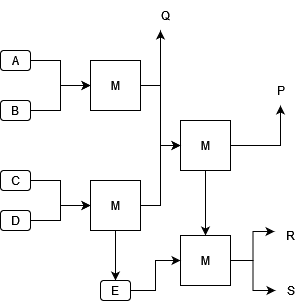
\includegraphics[width=0.6\textwidth]{images/mix.png}
\caption{An attack in mix networks. Here, M are the mixes and A, B, C, D, E are the senders.}
\label{fig:mix}
\end{figure}

Following this review we come to a conlcusion that we need a better metric to determine the quality of anonymity offered to the users. Serjantov et al. introduce entropy to describe quality of anonymity \cite{andreiInformation}. Entropy is a measure of the uncertainty of a random variable \cite{shannon}. In this scneario, the attacker has a probability distribuition, $P$, over the set of all participants with regards to them sending or receiving a message. They now define the effective size of the probability distribuition to be equal to the entropy of the distribuition: 
\begin{equation}
    \label{eq:entropy}
    S = -\sum_{u \in \Psi} p_u \log_2 p_u
\end{equation}
Here, $p_u$ is $P(u, r)$, $\Psi$ is the set of all participants and $r \in$ \{sender, recepient\}. This can also be interpreted as the number of bits of additional information required to identify a user of a particular message.




\section{Applications}
Idemix \cite{idemix} is an implementation of an anonymous credential system based on protocols described in \cite{Camenisch2001AnES}. The system offers an easy-to-use access control mechanism that can be integrated with user applications. The library needs to be imported into the application, and the application extends the library with its own access control policies.

For instance, the authors illustrate the system's utility in the context of a New York Times (NYT) news service subscription. In this example, a user first acquires a credential from a bank (ARGENTIX) for \$10, which is then shown to the New York Times news subscription service (KIOSK) to obtain another credential. The final credential is presented to NYT to get the subscription. Throughout these transactions, pseudonyms are used, and the process is unlinkable, thereby ensuring full anonymity for the user.

However, the system still requires an external trusted third party to issue root pseudonyms and credentials based on some verification of the user's real identity. To prevent credential sharing, the authors propose two types of safeguards: \textit{all-or-nothing}, where the user can share all or none of their credentials, and \textit{PKI-assured non-transferability}, which links a master secret to a valuable secret key from outside the system (e.g., he secret key that gives access to the user's bank account). The latter option is rarely available.

Optional anonymity revocation also requires a third party to reveal the pseudonym used for the transaction (local revocation) or reveal the user's real identity (global revocation). Both the user and the organization need to agree on the conditions that would lead to revocation (e.g., illegal transactions).

The system's implementation uses zk-proofs to validate user credentials, resulting in significant computational overhead on both the user and organization sides. The authors' benchmark results show that registering a pseudonym, issuing a credential, and showing a credential can take up to 25 seconds.



\bibliographystyle{IEEEtran}
\bibliography{bibliography.bib}

\end{document}